\documentclass{standalone}

\usepackage{tikz}
\usepackage{pgfplots}
\usetikzlibrary{calc}
\pgfplotsset{compat=1.15}

\begin{document}

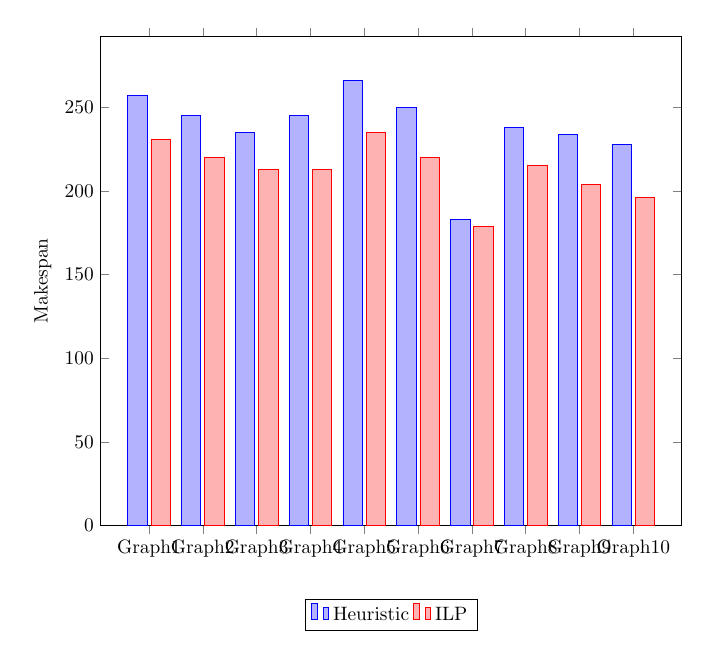
\begin{tikzpicture}[scale=0.7]
    \begin{axis}[
        width=\textwidth,
       % x tick label style={/pgf/number format/1000 sep=},
				symbolic x  coords={Graph1,Graph2,Graph3,Graph4, Graph5,Graph6,Graph7,Graph8,Graph9,Graph10},
        ylabel=Makespan,
				ymin=0,
        %enlargelimits=0.15,
        legend style={at={(0.5,-0.15)},
        anchor=north,legend columns=-1},
        ybar,
        bar width=10pt,
        ]
        \addplot
        coordinates {
				  (Graph1,257)
					(Graph2,245)
					(Graph3,235)
					(Graph4,245)
					(Graph5,266)
					(Graph6,250)
					(Graph7,183)
					(Graph8,238)
					(Graph9,234)
					(Graph10,228)
				};
        \addplot
        coordinates {
				  (Graph1,231)
  (Graph2,220)
  (Graph3,213)
  (Graph4,213)
  (Graph5,235)
  (Graph6,220)
  (Graph7,179)
  (Graph8,215)
  (Graph9,204)
 (Graph10,196)
				};
        
        \legend{Heuristic,ILP}
    \end{axis}
\end{tikzpicture}

\end{document}